\chapter{Digging into Concurrent Programming}\label{chap:cp_digging_into_concurrent_programming} % (fold)
\paragraph{Recalling Terminology}\label{par:cp_recalling_terminology} % (fold)
\begin{definition}{Concurrent Programming}{conc-prog}
    \textbf{Concurrent programming} consist of building programs in which multiple computational activities \textit{overlap} in time and typically interact in some way, without necessarily running on separate physical processors.
    It's placed at logical/abstract/programming level focusing on program organization.
\end{definition}
\begin{definition}{Parallel Programming}{para-prog}
    When the execution of programs overlaps in time by running on \textit{separate physical processes} is called \textbf{parallel programming}.
    It's placed at physical level focusing on performance.
\end{definition}
\begin{definition}{Distributed Programming}{distr-prog}
    \textbf{Distributed programming} occurs when processors are distributed over a network with no shared memory.
\end{definition}
\begin{description}
    \item[Multi-threaded programming] They have a shared state using synchronisation mechanisms (like semaphores, monitors, etc.)
    \item[Message-based programming] No shared state with interaction by means of message exchange (asynchronous vs synchronous)
    \item[Event-driven programming] The flow of the program is determined by events: user actions, sensors, messages from other threads/processes/apps
\end{description}
% paragraph Recalling Terminology (end)
%
\section{Concurrent Programming Performance}\label{sec:cp_concurrent_programming_performance} % (fold)
A \textbf{performance improvement} is achieved by:
\begin{itemize}
    \item increasing application \textbf{throughput} by exploiting parallel hardware;
    \item increasing application \textbf{responsiveness} by optimizing the interplay among CPU an I/O activities;
\end{itemize}
\begin{definition}{Speedup}{speedup}
    To measure performance the \textbf{speedup} is used, defined like this:
    \[
        S = \frac{T_1}{T_N}
    \]
    \begin{itemize}
        \item $N$ is the number of processors;
        \item $T_1$ is the execution time of sequential algorithm;
        \item $T_N$ is the execution time of the parallel algorithm using $N$ processors;
    \end{itemize}
\end{definition}
\subsection{Amdahl's Law}\label{sub:cp_amdahl_s_law} % (fold)
\begin{theorem}{Amdahl's law}{}
    The maximum speedup parallelizing a system:
    \[
        S = \dfrac{1}{1 - P + \dfrac{P}{N}}
    \]
    \begin{itemize}
        \item $P$ is the proportion of a program that can be made parallel;
        \item $(1-P)$ is then the part that cannot be parallelized;
    \end{itemize}
    \begin{note}[Theoretically maximum for $P = 1$ (linear speedup)]
        Actually there are specific cases with $S > N$ (super-linear) speedup
    \end{note}
\end{theorem}
\begin{cimage}
    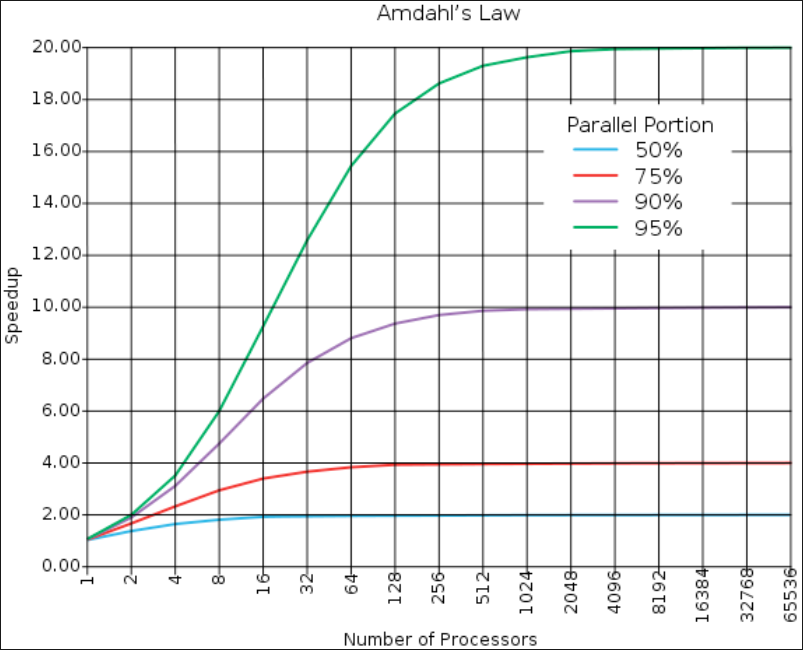
\includegraphics[width=.4\textwidth]{assets/20261012_120209.png}
\end{cimage}
\begin{remark}{}{}
    We can improve performance by adding processors only for those parts that can run in parallel, not for sequential parts $\rightarrow$ strong impact on performances of sequential parts.
    \begin{note}
        But sequential parts are often needed for correctness
    \end{note}
\end{remark}
\begin{definition}{Efficiency}{efficiency}
    Normalized measure of speedup indicating how effectively each processor is used:
    \[
        E = \frac{S}{N}
    \]
    \begin{itemize}
        \item $S$ is the speedup;
        \item $N$ is the number of processors;
    \end{itemize}
    \begin{note}
        The ideal efficiency is $1$, meaning all processors are used at full capacity (typically is lower)
    \end{note}
\end{definition}
\paragraph{A New Bottleneck: Memory}\label{par:cp_a_new_bottleneck_memory} % (fold)
Shared memory and bus as potential bottleneck: only one memory operation takes place at a time
\begin{note}
    Cache coherency protocol more and more complex and smart
\end{note}
\begin{cimage}
    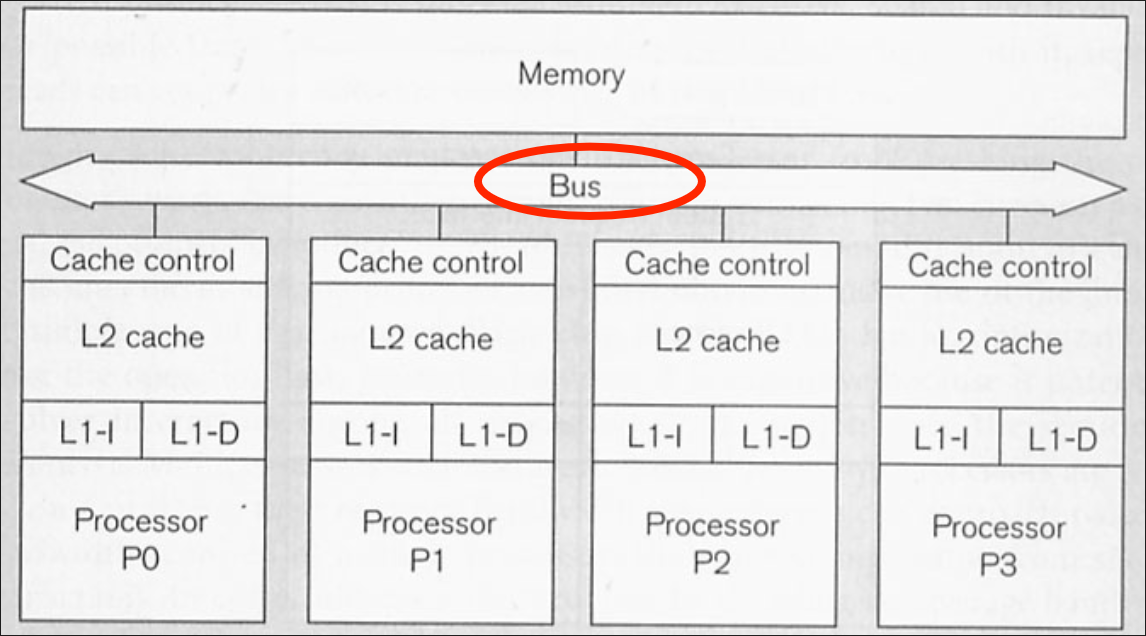
\includegraphics[width=.6\textwidth]{assets/20261012_130322.png}
\end{cimage}
% paragraph A new Bottleneck: Memory (end)
% subsection Amdahl's Law (end)
% section Concurrent Programming Performance (end)
%
\section{Design \& Abstraction}\label{sec:cp_design_abstraction} % (fold)
We define a proper level of abstraction for programs which interact with environment, control multiple activities and handle multiple events.
\begin{warning}[Objects from OOP are not enough]
\end{warning}
Concurrency is used as a tool for software design and construction, rethinking to the way in which:
\begin{itemize}
    \item we solve problems basic algorithm \& data structures;
    \item we design and build systems with a new level of abstraction: different kind of decomposition, modularization, encapsulation;
\end{itemize}
\begin{note}
    Affecting the full engineering spectrum: modelling, design, implementation, verification and testing
\end{note}
\begin{remark}{Processes}{ext-proc}
    A sequential program in execution, it is the basic unit of a concurrent system, single thread of control with logical thread of control/control flow, not necessarily physical.
    The sequence of instructions operating together as a group, dividing the work by \textit{unit of work} (\textbf{task}).
    \begin{warning}[Speed Independence]
        Process execution is meant to be completely asynchronous with each other: we can't do any assumption about their speed (\textbf{non-determinism})
    \end{warning}
\end{remark}
%
\subsection{Process Interaction}\label{sub:cp_process_interaction} % (fold)
\hyperref[def:process]{Process} interaction is a non-trivial concurrent program based on multiple processes that need to interact in some way.
The basic kinds of interactions are:
\begin{itemize}
    \item \textbf{cooperation};
    \item \textbf{competition}/contention;
    \item interferences;
\end{itemize}
%
\subsubsection{Cooperation}\label{sub:cp_cooperation} % (fold)
\begin{definition}{Cooperation}{cooperation}
    It refers to interactions which are both \textit{expected} and \textit{wanted}, they  are part of the semantics of the concurrent program.
\end{definition}
There are two basic kinds:
\begin{itemize}
    \item \textbf{communication}: concerns the need of releasing and information flow among processes, typically realized in terms of messages;
    \item \textbf{synchronisation}: concerns the explicit definition or presence of \textbf{temporal relationships} or dependencies among processes and among actions of distinct processes;
\end{itemize}
% subsubsection Cooperation (end)
%
\subsubsection{Contention/Competition}\label{sub:cp_contention_competion} % (fold)
\begin{definition}{Contetion/Competition}{cont-comp}
    It refers to interactions which are \textit{expected} and \textit{necessary}, but \textbf{not wanted}, typically it concerns the need of coordinating the access by multiple processes to shared resources.
\end{definition}
There are two basic class of problems:
\begin{itemize}
    \item \textbf{mutual exclusion}: ruling the access to shared resources by distinct processes;
    \item \textbf{critical sections}: ruling the concurrent execution of blocks of actions by distinct processes;
\end{itemize}
%
\paragraph{Synchronisation vs Mutual Exclusion}\label{par:cp_synchronisation_vs_mutual_exclusion} % (fold)
Two different concepts: \textit{synchronisation} is a mutual exclusion urban legend.
Synchronisation defines a \textit{timing relationship} among processes: maintaining \textbf{time-relationships} which includes actions happening at the same time or happening at the same relative rate or simply some action having to occur before another.
\begin{note}
    The mutual exclusion defines a \textit{restriction} on access to shared data: mutual exclusion is meaningless if no shared data is involved
\end{note}
\emptyln{}
Relationships:
\begin{itemize}
    \item mutual-exclusion typically require some forms of \textit{implicit synchronisation}, blocking some actions, waiting for other actions to complete;
    \item synchronisation does not necessarily require any kind of shared data and the mutual exclusion;
\end{itemize}
% paragraph Synchronisation vs Mutual Exclusion (end)
\paragraph{Difficulty of Synchronisation}\label{par:cp_difficulty_of_syncrhonisation} % (fold)
\begin{example}{}{}
    ``Alice and Bob live together, happily without cell-phones. Both are responsible to buy the milk when it finishes...''
    \begin{ctable}{|c|l|l|}
        \hline
        \textbf{Time} & \textbf{Alice} & \textbf{Bob} \\
        \hline
        5:00 & Arrive home & \\
        \hline
        5:05 & Look in the fridge: no milk & \\
        \hline
        5:10 & Leave for a grocery & \\
        \hline
        5:15 & & Arrive home \\
        \hline
        5:20 & & Look in the fridge: no milk \\
        \hline
        5:25 & Buy milk & Leave for grocery \\
        \hline
        5:30 & Arrive home: put milk in fridge & \\
        \hline
        5:40 & & Buy milk \\
        \hline
        5:45 & & Arrive home: oh no! \\
        \hline
    \end{ctable}
    Looking for a solution to ensure that:
    \begin{itemize}
        \item only one person buys the milk, when there is no milk;
        \item someone always buys the milk, when there is no milk;
    \end{itemize}
    \begin{note}[Tentative solution: using notes on the fridge]
    \end{note}
    \begin{codeblock}{}
    if (no note) then
        if (no milk) then
            leave note
            remove note
        fi
    fi
    \end{codeblock}
    \begin{critical}[It doesn't always work]
    \end{critical}
    \begin{ctable}{|c|l|l|}
        \hline
        \textbf{Time} & \textbf{Alice} & \textbf{Bob} \\
        \hline
        5:00 & Arrive home & \\
        \hline
        5:05 & Look at the fridge: no note & \\
        \hline
        5:10 & ... Ops! Need a toilet & \\
        \hline
        5:15 & ... Still in the toilet... & Arrive home \\
        \hline
        5:20 & ... Still in the toilet... & Look at the fridge: no note \\
        \hline
        5:21 & ... Still in the toilet... & Look in the fridge: no milk \\
        \hline
        5:22 & ... Still in the toilet... & Leave note \\
        \hline
        5:25 & ... Still in the toilet... & Go and buy milk \\
        \hline
        5:45 & Look in the fridge: no milk (*) & ... \\
        \hline
        5:50 & Leave note... & \\
        \hline
    \end{ctable}
    \begin{note}[(*)]
        Alice does not realize that a note was put on the fridge and strictly follows the established program
    \end{note}
\end{example}
% paragraph Difficulty of Syncrhonisation (end)
% subsubsection Contention/Competion (end)
%
\subsubsection{Interferences}\label{sub:cp_interferences_and_race} % (fold)
\begin{definition}{Interferences}{interf}
    It refers to interactions which are \textit{neither expected}, nor \textit{wanted}.
    They produce bad effects only when the ratio among the process speeds assumes specific values (time-dependent errors).
\end{definition}
\begin{definition}{Race Condition}{race-cond}
    \textbf{Race condition} or \textbf{race hazard} or simply \textbf{race}, whenever two or more processes concurrently access and update shared resources, and the result of the single update \textit{depends on the specific order occurring} in process access.
\end{definition}
Related to two main types of programming errors:
\begin{itemize}
    \item bad management of expected interactions;
    \item presence of spurious interactions not expected in the problem;
\end{itemize}
% subsubsection Interferences and Race (end)
%
\paragraph{Critical Situations}\label{par:cp_critical_situations} % (fold)
\hyperref[def:interf]{Interferences} and errors in \hyperref[def:conc-prog]{concurrent programs} can lead to \textbf{critical situations} for the concurrent system in the overall.
\begin{definition}{Deadlock}{deadlock}
    Situation wherein two or more competing actions (processes) are waiting for the other to finish, and thus neither ever does; typically concerns the release of a locked \textbf{shared resource}, the reception of a temporal signal or a message.
    \begin{critical}[It concerns multiple processes]
    \end{critical}
\end{definition}
\begin{definition}{Starvation}{starvation}
    Situation wherein a process is blocked in an infinite waiting.
    \begin{note}[Resource Starvation]
        The process is perpetually denied in accessing necessary resources
    \end{note}
    \begin{critical}[It concerns a single process]
    \end{critical}
\end{definition}
\begin{definition}{Livelock}{livelock}
    A \textbf{livelock} is similar to a \hyperref[def:deadlock]{deadlock}, except that the states of processes involved in the livelock constantly change with regard to another, none progressing.
\end{definition}
% paragraph Critical Situations (end)
% subsection Process Interaction (end)
% section Design \& Abstraction (end)
%
\section{Concurrent Machines}\label{sec:cp_concurrent_machines} % (fold)
To \textit{describe/specify} a concurrent program we need \textbf{concurrent programming languages} enabling programmers to write down programs as set of instructions to be executed concurrently.
\emptyln{}
To \textit{execute} a concurrent program we need a \textbf{concurrent machine}.
\begin{definition}{Concurrent Machine}{conc-machine}
    A \textbf{concurrent machine} is designed to handle the execution of multiple \hyperref[def:seq-process]{sequential processes}, by exploiting multiple processors (physical or virtual).
    \emptyln{}
    It provides:
    \begin{itemize}
        \item a support for the execution of \hyperref[def:conc-prog]{concurrent programs} and realizing then concurrent computations;
        \item as many virtual processors as the number of processes composing the concurrent computation; 
    \end{itemize}
    Providing basic mechanism for:
    \begin{itemize}
        \item \textbf{multiprogramming}: virtual processors generation and management;
        \item \textbf{synchronisation} and \textbf{communication};
        \item \textbf{access control} to resources;
    \end{itemize}
\end{definition}
\begin{definition}{Multiprogramming}{multi-prog}
    Set of mechanisms that make it possible to create new virtual processors and allocate physical processors of the lower-level machine to the virtual processors by means of scheduling algorithms.
\end{definition}
\begin{description}
    \item[Synchronisation and Communication] Two different typologies of mechanisms, related to two different \textit{architectural models} for \hyperref[def:conc-machine]{concurrent machines}:
        \begin{itemize}
            \item \textbf{shared memory model}, presence of a shared memory among the virtual processors (multithreaded programming);
            \item \textbf{message passing model}, every virtual processor has its own memory and no shared memory among processors is present.
                \begin{note}
                    Every communication and interaction among processors is realized through message passing
                \end{note}
        \end{itemize}
\end{description}
%
\paragraph{From Machines To Programming Languages}\label{par:cp_from_machines_to_programming_languages} % (fold)
Programming languages for specifying concurrent programs on top of \hyperref[def:conc-machine]{concurrent machines}: programs are organized as sets of \hyperref[def:seq-process]{sequential processes} to be executed concurrently on the virtual processors of the \hyperref[def:conc-machine]{concurrent machine}. 
\begin{note}[Basic constructs for:]
    \begin{itemize}
        \item \textbf{specifying concurrency}, creation of multiple processes;
        \item \textbf{specifying process interaction}, synchronisation, communication and mutual exclusion;
    \end{itemize}
\end{note}
% paragraph From Machines To Programming Languages (end)
% section Concurrent Machines (end)
% chapter Digging into Concurrent Programming (end)
